%---------------------
\section{Introduction}
%---------------------

% !TEX root = ./paper.tex
The Transmission Control Protocol (\tcp) \cite{rfc793} is one of the most critical protocols in today's Internet. A wide range of applications that require reliable delivery use it. During the last four decades, \tcp evolved under the pressure of competing protocols. During the 1980s, software-based \tcp implementations were considered too slow. Researchers proposed new transport protocols such as \xtp~\cite{sanders1990xpress} which could be implemented in hardware. Meanwhile, \tcp implementations got a considerable speed boost~\cite{clark1989analysis}, and \xtp did not succeed.  However,
the \tcp speed boost and usage triggered the development of various important \tcp extensions, including timestamps and large windows~\cite{rfc1323} to scale to the gigabit link speed or Selective Acknowledgments~\cite{rfc2018}.

During the late nineties, early 2000s, transport protocol researchers
explored other alternatives to \tcp. Two of these approaches were adopted
and standardized within the IETF: \dccp~\cite{kohler2006designing} and
\sctp~\cite{rfc4960}. We rarely use \dccp today. Despite its benefits
(support for multihoming, better design, and extensibility), only a few niche
applications use \sctp~\cite{budzisz2012taxonomy}. This limited deployment is probably due to two different factors. First, \sctp required changes to the applications to replace \tcp. Second, operators have deployed middleboxes (NAT, firewalls, etc.) that often block packets that do not carry \tcp or \udp~\cite{honda2011still}.

\sctp initially supported multihoming by switching from one path to another. It
was later extended to be able to use different paths continuously~\cite{iyengar2006concurrent}.  Multipath \tcp~\cite{rfc6824,raiciu2012hard} brought similar multihoming capabilitiy to \tcp, and included a coupled congestion control scheme~\cite{wischik2011design}, later brought to \sctp as well. This particular
succession of events shows how different designs can collaborate to advance each others.  Multipath \tcp is now deployed, notably on
smartphones~\cite{bonaventure2016multipath}. Other recent \tcp extensions include \tcp Fast Open~\cite{rfc7413} or TCPCrypt~\cite{rfc8548}.


%However, there are several limits to \tcp's extensibility. First, the
%entire \tcp header, including options, cannot be longer than
%64 bytes, which leaves a limited space to carry new options, in particular
%inside SYN packets. The IETF tried to circumvent this limitation
%\cite{draft-ietf-tcpm-tcp-edo-10}, but no \tcp stack has adopted it.
%Second, and more importantly, various
%deployed middleboxes make assumptions about the semantics of the \tcp
%packets that they process. Some of these middlebox, e.g. in mobile or
%satellite networks, transparently terminate \tcp connections initiated by
%client devices to optimise their performance. Others, like firewalls, analyse
%the packets exchanged to detect varioustypes of attacks.
%Unfortunately, many of these middleboxes block the \tcp options that they
%do not understand. This is affected the design of recent \tcp extensions like
%Multipath \tcp or Fast Open that has even been disabled by some vendors
%due to operational issues with middleboxes. This problem also
%affects other standardised transport protocols like DCCP \cite{} or
%SCTP \cite{} that already have difficulties to traverse simple middleboxes
%such as NATs.

In the mid-nineties, the Secure Socket Layer protocol was proposed to secure
emerging e-commerce websites~\cite{draft-hickman-netscape-ssl}. This protocol
evolved in different versions of the Transport Layer Security (\tls) protocol, the most recent one being version 1.3~\cite{rfc8446}. Many details of the \tls protocol have changed since the first version of SSL~\cite{kotzias2018coming}. Nowadays, \tls is almost ubiquitous on web servers~\cite{holz2019era} thanks to the availability of various \tls implementations and automated certificate authorities~\cite{aas2019let}. Furthermore, many non-web applications also rely on \tls~\cite{anderson2019tls}.

%In parallel, we also observe a growing deployment of \tls. A large fraction of
%the Internet traffic is currently composed of application data secured by \tls
%that is transported by \tcp. \tls brings several benefits from privacy and
%security viewpoints, but does not currently help with the middlebox problem.

Transport protocols continued to evolve in parallel. \quic started as
a proprietary protocol used by Google to speed up web
transfers~\cite{roskind2013quic,langley2017quic}. During the last years, it evolved into a complete transport protocol whose standardization is being finalized within the IETF~\cite{draft-ietf-quic-transport}. \quic combines the
functions that are usually found in \tcp, \tls, and HTTP/2. A key characteristic
of \quic is that it encrypts almost all the packets, including most of their headers. Although \quic is essentially a new transport protocol, it does not run
directly above IP in contrast with \sctp, \tcp, or \dccp. \quic runs above \udp. This choice is mainly motivated by the desire to avoid as much as possible
middlebox interference. \quic's clean architecture has attracted researchers
who have already proposed various extensions to the protocol~\cite{de2019pluginizing,viernickel2018multipath,polese2019survey,michel2019quic,draft-huitema-quic-ts,draft-shi-quic-dtp,draft-swett-nwcrg-coding-for-quic}.

Does the finalization of version 1 of the \quic specification mark the
end of the \tcp era and move all transport research on this new protocol?
We do not think so. History tells us that \tcp has evolved with competing
transport protocols. \quic is today's competitor, but there is still plenty of
room to improve \tcp.

In this paper, we take a step back. As \quic benefits from a closer integration between the reliability and the security mechanisms, we reconsider the separation between \tcp and \tls.
%By considering \tcp and
%\tls as independent protocols,  a very important opportunity.
\tls brings security features, but \tls 1.3 can do much more. Thanks to the \tls 1.3 messages and records' extensibility, \tls can provide a secondary channel that enables hosts to exchange more control information and structured data. Furthermore, since \tls records are encrypted, middleboxes cannot easily interfere with the data exchanged over this new channel.

%In this paper, we combine both \tcp and \tls in a single protocol called \textbf{\tcpls}. We describe in Sec.~\ref{sec:design} a first design for \tcpls with the goals of ($i$) solving extensibility issues in \tcp. ($ii$) Exporting complex transport features to the application and, ($iii$), drawing a path to make \tcp/\tls a good challenger to \quic with modern appications.   This paper also discusses how \tls flexible record layer can be used to provide a new channel to exchange information between \tcpls implementations. The design presentation concludes with an overview of the API to interact with the application.  Our second contribution is the ongoing
%implementation of a \tcpls prototype on Linux by extending \texttt{picotls}, a
%\texttt{TLS 1.3}
%implementation.  We use it in Section~\ref{sec:prototype} to illustrate the
%benefits of \tcpls with a multihoming connection migration use case. Finally, we analyze in Section~\ref{sec:research} some of the research questions that \tcpls opens.

In this paper, we combine both \tcp and \tls in a single fast, flexible, and secure protocol called \textbf{\tcpls}.  We have designed \tcpls with three goals in mind.  First, we aim at solving extensibility issues in \tcp \todo{BD: How? A quick word on that here would be appreciated}. Second, we export complex transport features, such as multipath capabilities \todo{BD: correct?}, to the application.  Finally, we draw a path to make \tcpls a good challenger to \quic. With that in mind, we have implemented \tcpls \todo{as a something in some library that will be made available upon the paper acceptance}.  It is also worth noticing that our implementation makes used of \tls flexible record layer so that it provides a new channel to exchange information between \tcpls information \todo{BD: provide here, with a few words, motivations and advantages of this additionnal channel}.  Finally, this paper evaluates the efficiency of our \tcpls implementation with respect to state of the art.  In particular, we demonstrate \todo{BD: summarize here the main measurements results}


The remainder of this paper is organized as follows: Sec.~\ref{sec:background} provides the required technical background; Sec.~\ref{sec:background-design} discusses how we designed \tcpls, while Sec.~\ref{sec:prototype} focuses on how we implemented \tcpls; Sec.~\ref{sec:evaluation} evaluates the performance and behavior of \tcpls;  finally, Sec.~\ref{sec:conclusion} concludes this paper by summarizing its main achievements and discussing further directions.

% Extending \tls's philosophy of protecting the transport layer (only Integrity,
% confidentiality and Authentication); now would also improve other issues of
% the transport layer.

%middlebox interferences

%The benefit of upgrading an individual endpoint depends on the number of other
%endpoints that have already been upgraded,since the new protocol is not
%effective unless both have it

% Talk about the backward-compatible nightmare when the security is at stake

% \tls offers an opportunity to fix part of \tcp's issues, offering a right
% abstraction of what a transport layer means for a given application.



%---------------------------------
%\section{Background \& Motivation}\label{sec:background}
%---------------------------------

%---------------------
\section{TCPLS Design}\label{sec:design}
%---------------------

\label{sec:background-design}
% Background and motivation

%TODO
%Gives an overview of \tls / \tcp and how they interact. We also need a comparison
%of QUIC and \tls/\tcp on several points that would serve as a base to explain why
%\tls 1.3's extensibility cannot compete with QUIC.
%Gives an overview of \tls / \tcp and how they interact. 

\tcpls offers a cross-layer interface to \tls and \tcp
with the motivation to do more than securing the transport layer. Merging the
stacks benefits both
protocols
and the application using this new approach. First, \tcp suffers from a lack of
extensibility due to size restrictions in its header and due to
potential middlebox interferences~\cite{honda2011still}. \tcpls aims to solve
\tcp's extensibility issue in the long run by offering a secure control channel
to exchange \tcp options without suffering from middlebox interferences and size restrictions in \tcp headers.
Second, \tls does not have a clear view of the transport protocol, and offering
one with \tcpls brings opportunity for performance improvement (e.g., avoiding
records fragmentation by matching the record size to the congestion window), and
for connection reliability (e.g., failover).  Third, applications are becoming
more complex, which appeals to exposing transport-level
functionalities and letting them tune the underlying transport to their use case.
Essentially, this last motivation discusses a novel manner to expose
transport-level functionalities that are encrypted, authenticated, reliable,
extensible and adapted to complex application-level requirements.
%The lack of
%extensibility impacts the design and deployability of new protocols, 
%such as \texttt{MP\tcp}~\cite{raiciu2012hard,rfc6824} or 
%\texttt{SCTP}~\cite{rfc4960}, and
%has motivated the design of QUIC~\cite{langley2017quic}.% and PQUIC~\cite{de2019pluginizing}.
%Therefore, designing a new extensibility mechanism could empower new
%application-level products and technologies. For these reasons, we design \tcpLS
%as an application-level configurable cross-layer wrapper for \texttt{\tls/\tcp} using
%\tls 1.3's extensibility mechanism to address \tcp's extensibility
%issues.
% High level vision
%To
%structure the discussion, we first focus on the establishment of a \tcpls
%connection. Then we discuss the exchange of data and the end of a connection. 


%\tcp uses a three-way handshake to establish a connection. Many server stacks
%generate the \synack directly from the \syn and only create state
%upon reception of the third \ack \cite{rfc4987}. \tcp extensions are 
%usually negotiated using \tcp options in the \syn and
%\synack packets. 
\subsection{Overview}

\tcp separates control information and data by placing the control information in
the packet header and the data in the payload. This separation worked well until
middleboxes started to interfere with \tcp~\cite{10.1145/1064413.1064418,
honda2011still, DHBVD13}.  On a fraction of Internet paths, including e.g., 
some enterprise and cellular networks, some middleboxes interfere by adding,
removing, or changing \tcp options \cite{wang2011untold, honda2011still, xu2015investigating} and, in some cases, also
transparently terminating \tcp connections. These middleboxes have slowed down
the evolution of \tcp in recent years. \tcpls also uses the packet header to
exchange \tcp control information, but it leverages \tls to create a second and
secure control channel. In a nutshell, \tcpls leverages the extensibility of \tls
1.3 to place control information such as \tcp options inside the \tls handshake
messages and new \tls records. Since this information is encrypted and
authenticated, the communicating hosts can exchange new control information
without encountering middlebox interference. We describe several examples of these new
types of control information in Section~\ref{sec:extending} and
Section~\ref{sec:connmigr}.


%A key benefit of \tcpls is that it leverages the encrypted parts of the \tls 1.3
%messages and records to create a new secure and independent channel between the
%communicating hosts. 

%interference that enables it to fallback to regular \tcp in the (expected rare)
%case of middlebox interference. This is similar to what Multipath \tcp does by
%sending its \syn with the \texttt{MP\_CAPABLE} initially and then removing this
%option after the third retransmission of the SYN \cite{raiciu2012hard}.

In our current prototype, a \tcpls session starts with a classic \tcp
handshake. Immediately after, the client sends the ClientHello \tls message. The
server replies with a ServerHello message which can contain encrypted data but
also encrypted control information. For example, a dual-stack server may
advertise its IPv6 address in the encrypted ServerHello message when contacted
over its IPv4 address. 
%Essentially, the \tcpLS handshake can become a control
%channel for goth \tcp and \tls. 
We highlight one of our roadmap features in
Section~\ref{sec:research} to enable a 0-RTT \tcpls which would enable \tcp to catchup
the QUIC design regarding fast connection establishment. We also describe in
Section~\ref{sec:content} how our current prototype uses this
information to support connection migration, failover, and other features.


%The \tcpls handshake can start with a \syn packet that contains a \tls
%ClientHello message inside its payload. This differs from the original \tcp
%handshake that does not usually include data in \syn packets.  We leverage the
%fact that the \tcp specification \cite{rfc793} allows a \syn to carry a payload
%and use it like the \tcp Fast Open extension (TFO) \cite{rfc7413}. As TFO,
%\tcpls uses cookies to counter attacks with spoofed packets, but these cookies
%are included in the ClientHello and can be much larger than those used by TFO.
%The server returns a \synack packet that contains the ServerHello message whose
%content is encrypted and authenticated. Since the ServerHello message is
%included in the payload, its length is not limited by a space requirement as in
%the \tcp header, but rather by a server choice of functionalities versus
%potential amplication attacks. It can contain additional information such as an
%identifier of the connection, the other addresses of the server or lightweight
%\tcp options such as a TCP User Timeout~\cite{rfc5482}.

%FR: this can be removed; it is almost a copycat at the end already
%In \tcpls, some \tcp options are sent in clear in the TCP headers
%while others can be encrypted. This brings two benefits.
%First, this hides those \tcp options from
%on-path middleboxes, including experimental ones \cite{rfc6994},
%that could be blocked. Second, \tcpls hosts can exchange over \tls
%records a summary of their state (initial sequence numbers, negotiated \tcp
%options, \ldots) to verify that their \tcp headers have not been tampered by
%middleboxes. Otherwise, they can fall back to regular \tls over regular \tcp
%to preserve connectivity as Multipath \tcp does it the MP\_CAPABLE
%option is stripped during the handshake \cite{rfc6824}.
%This could help to
%cope with some specific middleboxes that have affected the deployment
%of \tcp Fast Open \cite{paasch2016network}.

Once the \tcpls session has been established, \tcpls sends TLS records. Most of
these records contain application data transmitted by the client or
the server. The control channel between the client and the 
server enables \tcpls to support new features, such as streams. Indeed, applications such as HTTP/2 support multiple streams mapped to a single
\tcp connection. However, there are situations, e.g., to prevent head-of-line
blocking, where different streams should be mapped over other underlying \tcp
connections. With \tcpls, the client and the server can establish different
datastreams over a single \tcpls session. The data from all these streams is
encrypted using \tls. Furthermore, thanks to the \tcpls API, the client and the
server can map each data stream to an underlying \tcp connection.
Thus, a \tcpls session can be composed of one or more \tcp connections
similarly as a Multipath \tcp connection gathers subflows. Note that, if
the multipath mode is enabled, then a lost packet over one \tcp connection may
create HOL blocking since packets received on other streams may have to wait for
the lost packet to be properly reordered and delivered to the application. In
the case of the multipath mode not enabled, this problem would not happen, but
the application has to be careful to map application objects per stream, and not to
mix these objects among several streams since the ordering would not be
guaranteed.

%This channel is used to exchange \tcp options and other TCPLS control messages.
%\tcpls uses it also to exchange information about the client and server
%addresses. Indeed, it is also
%possible to attach another \tcp connection to complement the TCPLS session, and
%attach QUIC-like streams to those \tcp connections. This can
%be used by multihomed devices such as smartphones to establish one \tcp
%connection over each network interface to support the same \tcpls
%connection. 
To support data from a given datastream to be exchanged over several \tcp
connections, \tcpls includes its sequence numbers. A client and server can also
enable acknowledgments. Thanks to these \tcpls
acknowledgments, a \tcpls session can react to the failure of the underlying
\tcp connection by reestablishing a new \tcp connection to continue the transfer
of data and replay the records that have been lost.
%This is similar to the handover capability of Multipath \tcp.

A \tcp connection ends with the exchange of \fin or \rst packets. However,
some middleboxes force the termination of \tcp connections
by sending \rst packets~\cite{rfc3360,weaver2009detecting}. \tcpls
can preserve established connections by automatically restarting
the underlying \tcp connection upon reception of a spurious reset. \tcpls
defines the connection termination at the stream level: closing the last stream
attached to a \tcp connection allows clients and servers to securely
terminate the \tcpls session.


%Todo explain that the transport abstraction level failed to offera versatile
%usage
%of the transport layer, and explain how a session layer can repair the
%abstraction
%Besides, with our design of \tcp extensibility
%within \texttt{\tcpLS}, applications would be able to tune \tcp on a connection basis,
%using existing options or any future option without middlebox interferences. As
%a matter of example, our \texttt{\tcpLS} implementation supports several
%\tcp options that can difficulty live at the \tcp layer
%(e.g., Joining a Multipath connection, injecting eBPF bytecode to the kernel's
%peer to tune \tcp). With \texttt{TCPLS}, we show how to solve several of these
%existing problem.

%Finally, \texttt{\tcpLS}'s control channel is expected to offer extensibility
%without middlebox interference and with protocol message indistinguishability
%from the network to avoid fingerprinting of the client stack. Our objective is
%to design a versatile \tcp extensibility mechanism that would allow to set
%options, exchange eBPF bytecode~\cite{de2019pluginizing} to tune the peer's kernel and implement new
%session behaviours.




% !TEX root = ./paper.tex

\subsection{\tcpls Transport Services}
\label{sec:transport-services}

%\todo{parler de secure control channel ? (mp): Pour moi non, c'est une vue de
%l'esprit, ça équivaut a dire qu'on peut utiliser des nouveaux records tls}

By leveraging \tcpls records and extensions, we can design new modern transport
services atop the combination of \tcp and \tls. In this subsection, we answer 
our second research question {\small\textit{RQ2}} by presenting three transport 
services: stream multiplexing (Section~\ref{sec:datastreams}), connection 
migration (Section~\ref{sec:multipath}), and bandwidth aggregation 
(Section~\ref{sec:multipath}). We leverage the \tcpls records
to multiplex concurrent encrypted bytestreams. By extending the \tls handshake, \tcpls allows joining several \tcp connections to a single \tcpls session to support
connection migration and %multipath capabilities, mitigating Head-of-Line
%blocking and enabling
bandwidth aggregation.
%aggregation and Head-of-Line blocking resilience.

\subsubsection{Stream Multiplexing}\label{sec:datastreams}
%%%%%%%%%%%%%%%%%%%%%%%%%%%%%%%%%

\begin{figure}[!t]
	\centering
	\begin{bytefield}[bitheight=\widthof{aw}]{32}
		\bitbox[]{1}{\small N} & \bitbox[]{9}{} & \bitbox[]{3}{\small N-32} &
		& \bitbox[]{7}{} &
		\bitbox[]{1}{\small 64} & \bitbox[]{9}{} & \bitbox[]{3}{\small 0} \\
		\bitbox{32}{TLS 1.3 AEAD Initial Vector}  \\
		\bitbox[]{12}{+} & \bitbox[]{8}{} & \bitbox[]{12}{$\oplus$} \\
		\bitbox{12}{\tcpls Stream ID} & \bitbox[]{8}{} & \bitbox{12}{Record sequence}
	\end{bytefield}
	\caption{The AEAD IV of \tcpls Streams is derived from \tls 1.3}
	\label{fig:aead-iv}
\end{figure}

Stream Multiplexing is a transport service that has been part of recent
protocols such as \sctp~\cite{rfc4960}, \quic~\cite{rfc9000} and HTTP/2.0
\cite{rfc7540}. The latter also proposes multiplexing with an independent
framing system atop the \tls-encrypted \tcp bytestream. In \tcpls, we choose to
implement multiplexing with \tcpls records. We dedicate a \tcpls record type to
\tcpls stream data. Each stream has a separate cryptographic context allowing
concurrent encryption and decryption of data within the same session.  A \tcpls
stream consists of a sequence of \tcpls stream data records encrypted with their
cryptographic contexts. Each stream is attached to one \tcp connection.

One simple way to provide separate cryptographic contexts is to use multiple
application-level keys. But this is known to degrade the security properties
proportionally to the number of additional keys~\cite{chatterjee2011another}. To
overcome this, we propose an Initial Vector (IV) derivation technique that
enables independent encryption/decryption to each stream without the security
degradation.

Figure~\ref{fig:aead-iv} illustrates how the AEAD IV is computed for a given
\tcpls record of a \tcpls stream. First the left-most bits of the IV derived
from the \tls handshake are summed with the 32-bit \tcpls Stream ID. Then the
right-most bits are XORed with the stream 64-bit record sequence number. Each
\tcpls stream has a separate record sequence number space. This combination of
IV manipulation guarantees that the resulting IV is unique for each record of
all \tcpls streams as long as the Stream ID is unique and no sequence number is
used twice in a given stream. The Stream ID space is split between the client
and the server. Stream ID 0 is equivalent to the cryptographic context directly
derived from the handshake.
%\todo{Il faut expliquer comment les stream id sont choisis pour garantir
%l'unicité}

To avoid possible middleboxes interference, in addition to the record sequence
number, the \tcpls Stream ID is kept implicit as well. When an endpoint receives
a \tcpls record, we leverage the AEAD cipher to check the authentication tag
repeatedly until the correct \tcpls Stream ID is found. An optimized
implementation would not involve a complete decryption as all TLS 1.3 AEAD
ciphers use an Encrypt-then-MAC construct~\cite{rfc7366, rfc8446}, and the tag
verification, especially on AES-GCM is computationnaly light.
%\todo{citer rfc7366 ? ou les références de ce rfc ?}

From a security standpoint, each failed decryption is considered as a forgery
attempt. However, the limits on confidentiality and integrity for AEAD ciphers
are large before a successful forgery may be considered with non-negligible
probability~\cite{luykx2015limits, aeadlimits}. For example, in the case of
ChaCha20 + Poly1305, an adversary making $2^{60}$ forgery attempts succeeds with
probability $2^{-33}$.
%\todo{Should we mention that one stream cannot be used on two connections at the same time?}

%The classical solution to support streams in a transport protocol is to assign
%an identifier to each stream and send the data from stream $x$ as a tuple
%$x,seq,data$ where $seq$ is a sequence number. This is the solution chosen by
%\sctp~\cite{rfc4960} and \quic~\cite{draft-ietf-quic-transport}. \tcpls relies
%on cryptographic properties to support several streams.

%\paragraph*{Cryptographic Details and Tricks} In \tcpls, each stream has its own
%cryptographic context. All streams use the same key but derive a specific
%Initial Vector (IV - also called cryptographic nonce) such that nonce-misuse
%cannot happen. Furthermore, \tcpls derives the IV such that the record sequence
%numbers can securely start at $0$ within each stream.
%
%\tcpls uses only one application-level key for $N$ streams, for each direction.
%We selected this approach to avoid security degradation with the usage of
%multiple keys (by a factor $k$ with $k$ keys)~\cite{chatterjee2011another}.

%To enable all stream sequence numbers to start at 0, we rely on some properties
%of the Authenticated Encryption with Associated Data (AEAD) schemes used by \tls
%1.3. To preserve AEAD security, the AEAD nonce used by \tcpls must be of unique
%use when encrypting and decrypting a record. The initial nonce must also be
%unpredictable for an adversary observing the handshake. \tcpls derives it from
%the \tls handshake session secret in a similar fashion to the \tls
%keys~\cite{rfc8446}. The nonce size ranges from $96$ bits to $128$ bits
%depending on the underlying cipher used. In all cases, for a nonce of size $N$
%bits, \tls computes the cryptographic nonce by concatenating the $N-64$ leftmost
%bits with the 64 lower bits XORed with the record's implicit sequence number
%encoded in 64 bits. XORing the lower 64 bits provides more unpredictability to
%the nonce when the same plaintext is encrypted multiple times with the same
%key~\cite{bellare2016multi,hoang2018multi}. This design implies that we give to
%the underlying cipher the 32 upper bits untouched. The resulting value is then
%concatenated with an internal counter in GCM and used as the blocksize-bits (128
%or 256 bits) stream's counter.
%We observe that the leftmost N-64 bits are available to encode a unique stream number. By
%encoding such a unique number in this part of the cryptographic nonce, we enable
%each stream to start its sequence number at 0 while encrypting its records with
%the same key. This observation means that we can create independent
%cryptographic contexts based on a cryptographic nonce's tweak. This implies
%that stream records can be encrypted and decrypted independently of each other,
%with the same key value. This technique maintains AEAD's core assumption
%(uniqueness of nonce), which means that state of art AEAD's security proof
%starting from that assumption applies to our
%design~\cite{chatterjee2011another} and guarantees the security of our scheme.

%\paragraph*{Carrying Multiple Streams over the Same Transport}
%(mp): TODO Multicore decryption could be listed as an improvement
%Thanks to those separate cryptographic contexts, \tcpls can perform concurrent
%encryption and decryption between streams while maintaining decryption
%correctness and security, and potentially also use this capability to process
%different streams over different CPU cores.
%Finally, when different streams are carried
%over the same \tcp connection, \tcpls does not explicitely know which stream
%a received record belongs to. To retrieve this information,
%we also
%leverage the AEAD cipher and check the incoming record's authentication tag
%until we find the stream that properly verifies this tag. This operation is
%lightweight: it does not require full decryption of the record because the AEAD
%ciphers used by \tls 1.3 do Encrypt then MAC (and MAC then Decrypt).
%Looking for the right stream that succeeds the tag verification needs to be
%performed once each time the application writes to another stream over the same
%\tcp connection.
%
%Note that, security-wise, each failed decryption is considered a
%forgery attempt. However, we have large limits on the confidentiality and
%integrity with all AEAD ciphers~\cite{luykx2015limits, aeadlimits} before a
%successful forgery may be considered as a non-negligible probability. For
%example, in the case of ChaCha20 + Poly1305, an adversary making $2^{60}$ forgery
%attempts succeeds with probability $2^{-33}$.


\subsubsection{Connection Migration}\label{sec:multipath}

\tcpls allows joining several \tcp connections to an existing \tcpls session.
We leverage this mechanism to implement new transport services such as connection migration. Compared to the subflow joining mechanism of
\mptcp~\cite{raiciu2012hard,hesmans2015smapp,hesmans2016enhanced}, our design is
more secure. Indeed, \mptcp supports additional subflows by initially exchanging
short keys inside cleartext \tcp \texttt{Options} during the \tcp handshake~\cite{rfc6824, rfc8684}. These keys are then used to authenticate the association of subflows. An attacker having observed the key exchange during the \tcp handshake can associate subflows to an existing \mptcp connection~\cite{rfc6181}.

\begin{figure}[!t]
	\centering
	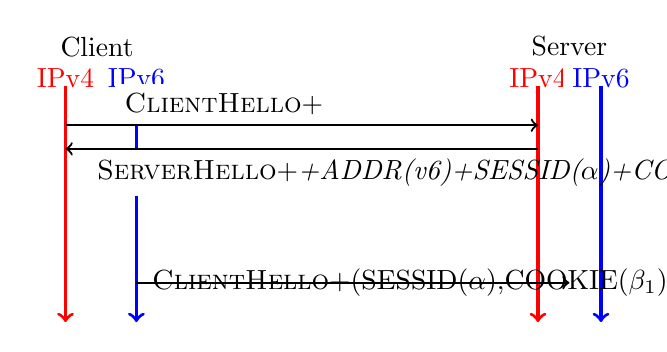
\begin{tikzpicture}
		\colorlet{lightgray}{black!20}
		\tikzstyle{arrow} = [thick,->,>=stealth]
		\tikzset{state/.style={rectangle, dashed, draw, fill=white} }
		\node[black, fill=white] at (0,10) {Client};
		\node[black, fill=white] at (6,10) {Server};
		\node[red, fill=white] at (5.6,9.6) {IPv4};
		\node[blue, fill=white] at (6.4,9.6) {IPv6};
		\node[red, fill=white] at (-0.4,9.6) {IPv4};
		\node[blue, fill=white] at (0.5,9.6) {IPv6};
		\draw[red, very thick,->] (-0.4,9.5) -- (-0.4,6.5);
		\draw[blue, very thick,->] (0.5,9.5) -- (0.5,6.5);
		\draw[red, very thick,->] (5.6,9.5) -- (5.6,6.5);
		\draw[blue, very thick,->] (6.4,9.5) -- (6.4,6.5);
		\draw[black, thick, ->] (-0.4,9) -- (5.6,9) node [midway, fill=white, above,
		text width=4.5cm] {\textsc{ClientHello}+\hello};
		\draw[black, thick, <-] (-0.4,8.7) -- (5.6,8.7) node [pos=0.5, fill=white, below, text width=5.2cm] {\textsc{ServerHello}+\emph{\hello+ADDR(v6)+SESSID($\alpha$)+COOKIE($\beta_1,\beta_2$)}};
		\draw[black, thick, ->] (0.5,7) -- (6.0,7) node [pos=0.4, %fill=white, above,
		text width=4cm] {\textsc{ClientHello}+\join(SESSID($\alpha$),COOKIE($\beta_1$))};
	\end{tikzpicture}
	\caption{\tcpls supports joining additional \tcp
		connections to a \tcpls session. The $SESSID$ and $COOKIE$ in the \textmd{\textsc{ServerHello}} are encrypted with the
		handshake key.}
	\label{fig:join-example}
\end{figure}

\textbf{Joining \tcp connections}. \tcpls leverages \tls
extensions to solve this problem in a more secure manner. 
Figure~\ref{fig:join-example} illustrates the \tls and \tcpls messages 
exchanged when a client connects to a server over IPv4 and later joins another 
connection over IPv6.
First, the client sends a \textsc{ClientHello} containing a \hello. The server 
replies with a \textsc{ServerHello} containing three encrypted extensions. 
First, the server announces its IPv6 address ($ADDR(v6)$). Second, it 
associates one identifier $\alpha$ to the \tcpls session 
(\emph{SESSID($\alpha$)}).
%It uniquely identifies the \tcpls session on the server.
Third, the server provides a list of \tcpls session cookies $\beta_1,\beta_2$ in the \emph{COOKIE} extension. Each of these session cookies enables the client
to join one additional \tcp connection to the \tcpls session. Thus by 
sending $n$ cookies over a session, the server restricts the client to 
join up to $n$ \tcp connections. This prevents resource exhaustion attacks
that are difficult to counter with \mptcp. The server can later send additional
cookies and update its list of addresses.

To join a new \tcp connection to the \tcpls session, for instance over IPv6, the
client sends a \textsc{ClientHello} message containing the session identifier
(SESSID($\alpha$) in Figure~\ref{fig:join-example}) and one of the cookies
provided by the server (COOKIE($\beta_1$) in Figure~\ref{fig:join-example}). The
server uses the session identifier $\alpha$ to find the corresponding \tcpls
session and checks the validity of the cookie. If the \tcpls session and cookie
are valid, the \tcp connection is joined to the \tcpls session. The session
identifier plays the same role as the \mptcp token, but is sent encrypted. The
cookie provides stronger protection than \mptcp's HMAC with security keys
exchanged in cleartext. The \tcpls cookies are sent encrypted by the server and 
can only be used once by the client.
%(i.e.,
%when the server receives a valid cookie, it accepts the connection, attaches it
%to the right \tcpls session, and discards the cookie).


%\tcpls includes a Connection Manager (CM) that controls the underlying \tcp
%connections.
%The CM is fully configurable and exposed to applications through the \tcpls API.
%\tcpls enables the client or the server to associate new \tcp connections to an
%existing \tcpls session. This is similar to \mptcp's path
%managers~\cite{raiciu2012hard,hesmans2015smapp,hesmans2016enhanced},
%but with some differences. First, \tcpls does not suffer from the same
%security limitations as \mptcp. Second, \tcpls supports several multipathing
%modes, including connection failover, bandwidth aggregation and non-aggregated
%multiple paths.

%\paragraph*{1) Better Security Than \mptcp} A \mptcp connection gathers several
%underlying connections called subflows. To ``secure'' the attachment of
%additional subflows, \mptcp hosts exchange short keys in plaintext inside \tcp
%options during the \tcp handshake~\cite{rfc6824, rfc8684}. These keys are then
%used later to authenticate the attachment of subflows. An
%attacker that has observed the initial handshake can attach any subflow to an
%existing \mptcp connection~\cite{rfc6181}. \tcpls leverages its secure channel
%to solves this \texttt{``connection join''} problem in a more secure
%manner. Consider a client connecting to a dual-stack server
%(Figure~\ref{fig:join-example} depicts the \tls messages exchanged in such a
%scenario). The client sends a \textsc{ClientHello} containing the \tls
%extension to negotiate \tcpls. The server replies with a \textsc{ServerHello}
%with three types of encrypted extensions. First, the server announces its IPv4
%and IPv6 addresses. Second, it associates one identifier to the \tcpls session
%(SESSID($\alpha$) in Figure~\ref{fig:join-example}). It uniquely
%identifies the \tcpls session on the server. Third, the server provides a list
%of \tcpls session cookies (COOKIE($\beta_1,\beta_2$) on
%Figure~\ref{fig:join-example}). Each of these session cookies enables the 
%client
%to attach one additional \tcp connection to the \tcpls session. By sending $n$
%cookies, the server indicates that it currently accepts the attachment of only
%$n$ \tcp connections to this session. This prevents resource exhaustion attacks
%that are difficult to counter with \mptcp. The server can send additional
%cookies later and update its list of addresses.
%
%To attach a new connection, e.g., using the server's IPv6 address, the client
%sends a \textsc{ClientHello} message containing the session identifier
%(SESSID($\alpha$) on Figure~\ref{fig:join-example}) and one of the server's
%cookies (COOKIE($\beta_1$) on Figure~\ref{fig:join-example}). The server checks
%the validity of the cookie and then uses the session identifier to attach the
%new \tcp connection to the right \tcpls session. The session identifier and
%cookie play that same role as \mptcp's token. From a security viewpoint, \tcpls'
%session cookie is longer than \mptcp's token. Furthermore, it is sent encrypted
%in the initial \textsc{ServerHello} message, and can only be used once (i.e.,
%when the server receives a valid cookie, it accepts the connection, attaches it
%to the right \tcpls session, and discards the cookie).

\begin{figure}[!t]
	\begin{center}
		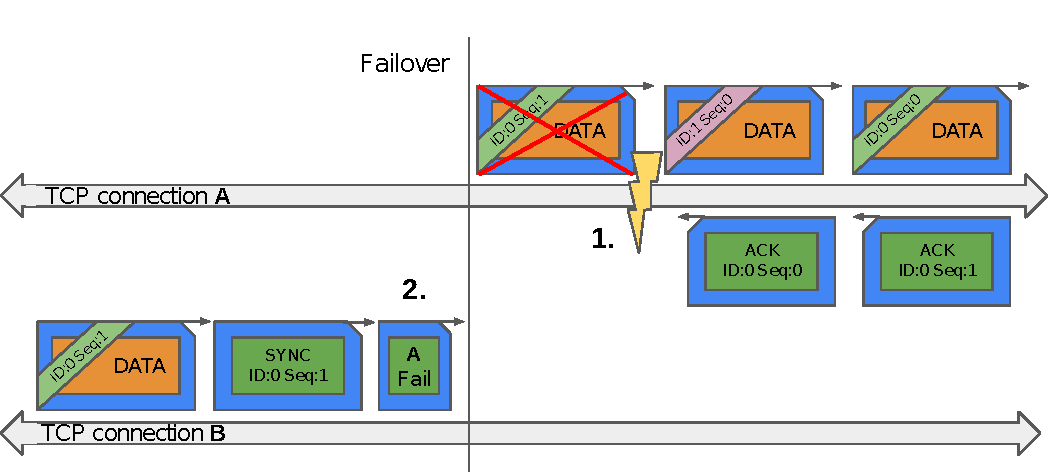
\includegraphics[width=\columnwidth]{figures/tcpls_failover}
	\end{center}
	\caption{Failover resynchronises and retransmits lost \tcpls records 
	from a failed \tcp connection to an other.}
	\label{fig:failover}
\end{figure}

\textbf{Failover}.
When a \tcp connection fails, e.g. due to middleboxes or network outages, 
\tcpls leverages its joining mechanism to recover 
the session over another \tcp connection. Figure~\ref{fig:failover} illustrates 
how \tcpls reacts to such events during a transfer with two \tcpls streams.
To achieve such a \emph{break-before-make}, 
\tcpls sends acknowledgments for the received records of each stream, allowing
the sender to remove them from its sending buffer.
%Upon reception of Stream-level acknowledgments, the sender can
%manage its sending buffer and remove acknowledged encrypted records. 
When the \tcp connection fails, the sender switches to the other one and 
explicitly notifies the failure to the receiver. The sender then synchronizes 
the transmission sequence using a dedicated \tcpls record type (i.e. SYNC in 
Figure~\ref{fig:failover}) and retransmits the 
unacknowledged stream data records (i.e. the second record of stream 0 in 
Figure~\ref{fig:failover}). 
Explicit synchronization %is required as the \tcpls stream sequence number is 
%implicit and thus 
prevents a lost acknowledgment from desynchronizing the endpoints. 
Thanks to the per-stream cryptographic context, the ciphertext of lost stream 
data records can be retransmitted as is.

%Furthermore,
%the unacknowledged data records sent over the failed \tcp connection are
%transmitted again over a functional one. To resynchronize the session (i.e., 
%the
%implicit encryption/decryption sequence numbers), the
%failover protocol makes the client sends the sequence number of the first 
%record
%within its sending buffer, an $id$ to specify the failed \tcp connection and
%the Stream ID of the stream being moved. This information is encrypted with
%the default context and sent within the new \tcp connection. Receiving this 
%protocol message, the server now knows
%the sequence number to decrypt some record arriving next on the connection that
%read the failover message. Either the server already processed that record, 
%and can safely
%ignore it and increase the sequence number, or the server did not yet seen that
%record, and can decrypt and process it. The same protocol message and 
%operations
%then goes from the server to the client, and the stream is then resyncronized
%over a new \tcp connection. No messages are required to be encrypted twice.
%\tcpls' Failover mode is optional. Both peers need to activate it or
%negotiate the feature throught the Secure Control Channel.
We present in Section~\ref{sec:perf} measurements quantifying the
performance impact of adding \tcpls record-level acknowledgments. We also
present in Section~\ref{sec:eval_failover} an analysis of recovery speeds during
different type of outages.
%We also give a
%trace example involving a file transfer and the failover protocol in
%Appendix~\ref{app:failover}.
%\todo{Let see if we can bring it back in the text later}

\textbf{Application Connection Migration}. \tcpls also enables the
application to trigger a connection migration, for instance based on application-level metrics qualifying its experience over the current path.
%expected to be used
%over
%healthy networks. %and leveraging a transient usage of bandwidth aggregation.
%(mp): I would leave this aside for now, until we explain application streams.
%The decision to migrate from a healthy network to another one is a
%application one.
%(mp): Yet the following meta-info are not described, and again implementation
%-> section
%4
\tcpls enables the exchange of meta-information to help this
decision.
%The TCPLS protocol and implementation's job is to make it quite simple by
%supporting the exchange of interface's related meta-information to help the
%decision
%making and by offering a simple API.
%Essentially, it means that \tcpls provides a simple API that enables an
%application to migrate when it wishes to do so (e.g.,
For instance, an interactive application running on a smartphone could migrate 
from
LTE to Wi-Fi when it senses an increase in delays due to bufferbloat for a
given period of time, or when a mobile client detects its home Wi-Fi and the
user's preference is to move its traffic to the Wi-Fi if detected.
%when the Wi-Fi appears healthy,
%The semantic of
%the application-level connection migration is built from attaching and closing
%streams in the multipath bandwidth aggregation mode.
%The client that wishes to
%carry such a migration first creates a new \tcp connection and joins the \tcpls
%session over this connection.
To achieve it, the client moves all its \tcpls streams to another \tcp
connection.
%(mp): avoid introducing concepts we define later rather than earlier
%can essentially use Stream Streering, i.e., the client
%\textit{composes} with independent
%features offered by \tcpls.
%(mp) -> section 4
%In a client/server implementation using \tcpls, the
%following protocol composition is realised with only 4 API calls (4 lines of
%code).
First, it creates a new \tcp connection and joins it to the
\tcpls
session. Then, %it steers the \tcpls stream abstraction,
it attaches new streams to the new
connection
%using the stream opening protocol
and removes the old ones from the underperforming connection, effectively moving
the application traffic to the new connection.
%(mp): Lets talk of that in the following section rather
%This stream steering
%mechanism may temporally takes advantage of bandwidth aggregation during the
%fraction of seconds required to open the second stream and close the first one.
%These properties are latter demonstrated in Section~\ref{sec:app-migration}.

%by sending one \textsc{Stream\_Attach} message per stream that needs
%to be migrated. At that moment, the client and the server have potentially
%multiple streams opened over the two network paths and can temporally aggregate
%the bandwidth offered by both paths. Then, after having attached
%all its streams to the new path, the migrating host sends a
%\textsc{Stream\_Close} message over the old \tcp connection for all old streams.
%At this point, the migrating host cannot send new stream data anymore over the
%old connection. Once the remote host has received a \textsc{Stream\_Close}
%message over the old \tcp connection, it knows that the connection is not
%available anymore\todo{?}, and can switch to the other connections. It first sends a
%\textsc{Stream\_Close\_Ack} message for each received \textsc{Stream\_Close}.
%The migrating host can close the old connection upon reception of the last
%\textsc{Stream\_Close\_Ack}, indicating that no more data would be received over
%this connection. Note that these messages are \tls records and are thus sent
%securely and reliably.% by the underlying \tcp connection.

This second type of migration does not require application-level
acknowledgments, but it cannot survive from one of the
underlying connections' failure. During such a migration, data may be sent over
two connections, which brings us to explain how multipath is designed.

\subsubsection{Multipath capabilities}

Like \mptcp, \tcpls allows an application to control different \tcp connections
that are used to exchange data. \mptcp was designed to be a drop-in replacement
for \tcp. A regular application that uses the socket API can use \mptcp without
any modification. \mptcp uses a path manager to control the underlying \tcp
connections. Several path managers were proposed in the Linux kernel
implementation \cite{TODO}.\todo{ref} However, few advanced applications have taken
advantage of these advanced path managers. Apple's \mptcp stack was tuned for
specific applications. For example, the Siri voice recognition application can
use both cellular and Wi-Fi to optimize performance. Apple Music mainly uses 
\mptcp to perform seamless handovers. As applications have very different 
requirements, \tcpls
exposes the underlying \tcp connections to the application through its API. The
applications use this API to implement their own policy to manage the
underlying \tcp connections.

%(mp): It's already part of related work actually
%When several networks paths are used in a transport
%connection, the congestion controller of each path should be coupled to control
%the overall aggressiveness of the connection. This problem has been solved in a
%generic way for MPTCP~\cite{rfc6356}, and the same solution could be applied to
%\tcpls. eBPF could be leveraged to access and modify the congestion controller
%state. We leave this engineering effort as future work.

\textbf{Stream Steering}. \tcpls enables the application to combine
multiplexing with the ability to join
several \tcp connections to a \tcpls session. This allows the application to
steer \tcpls
streams over the different \tcp connections. While Failover moves
\tcpls streams from one connection to another when a \tcp connection fails, stream
steering allows the application to distribute at any time the streams over the
different
\tcp connections of a \tcpls session. We already discussed a very simple use of
stream steering when performing Application Connection Migration %, which plays
%with opening, attaching and closing \tcpls stream protocols 
to move application data to a new connection.

%Like \mptcp \cite{raiciu2012hard,rfc6824} or Multipath QUIC
%\cite{de2017multipath,draft-liu-multipath-quic-02}, \tcpls supports an
%aggregation mode that maps data over two or more \tcp connections. On multihomed
%hosts, this can increase the total throughput of a \tcpls session by spreading
%the data over different network interfaces. In this case, one or more data
%streams are mapped to two or more underlying \tcp connections and \tcpls
%schedules different records over different connections.

Applications assign \tcpls streams to \tcp connections through the \tcpls
API.
%The choice of assigning to the \tcpls streams to the \tcp connections is left
%to the application through the \tcpls API.
An interactive game could use different streams for chat messages and player's
commands.  Also, an HTTP server could choose
the \tcp connection for the stream of each response based on the content type of
the response. Latency-critical objects could be sent over
low-latency connections. By sending each application-level object in a separate
stream, the application can benefit from multiple network paths while
maintaining the ability to process each stream in a zero-copy manner, and
with no head-of-line blocking.
\tcpls enables the application to choose which streams are protected from
Head-of-Line blocking by placing them on separate \tcp connections.
%Applications objects that depend on others can cope with occasional
%Head-of-Line blocking.

%\todo{Choix du HoL, ça coute des connexions mais pas forcément nécessaire en
%	fonction de l'app.}

%\todo{OB: paragraphe ci-dessous pas clair. (mp): C'est m-à-j}
%\todo{Multipath congestion control appliqué a TCPLS, eBPF, pas trivial}

\textbf{Coupling streams for aggregated bandwidth}. 
%Recall that each stream isbattached to only one \tcp connection. 
Applications that benefit
from the aggregated bandwidth of several network paths when transmitting a
single application object can use \tcpls \textit{coupled streams}. Coupled
streams send data alongside a sequence number located at the end of
the record. The sender can schedule \tcpls records of an application
object over these streams and benefit from their aggregated bandwidth by 
sending data over the two streams using a strategy that fits the application 
usage. The receiving application reads the application object in order, as 
\tcpls handles the reordering of coupled streams decrypted records.
%That is, with coupled streams, \tcpls offers
%to the application an explicit interface to the sender, and an agnostic
%interface to the receiver
%This provides a level of service similar to MPTCP and MPQUIC.

Dozens of packet schedulers were proposed for \mptcp. The default one is the
RTT-based scheduler that favors the subflow with the lowest RTT
~\cite{paasch2014experimental}. Other schedulers include the redundant
scheduler
that sends data over both subflows~\cite{frommgen2016remp}, schedulers that
help to minimize reordering on the receiver side~
\cite{lim2017ecf,hurtig2018low}, schedulers specialized for mobile
applications~\cite{de2018tuning}, \ldots
The most flexible approach remains the application-defined Multipath TCP
scheduler~\cite{frommgen2017programming}, but this solution has never been
integrated in \mptcp implementations.

\tcpls takes a different viewpoint. It exposes the underlying \tcp connections
and the sender side \tcpls record scheduler to the application. This enables
the application to actively decide the \tcp connection that it will use to send
each record. A remote terminal application running over \tcpls could send the
screen updates over a high bandwidth but high latency connection and the
keyboard input over the lower latency one.
%(mp): On ne peut pas il me semble
Using socket options such as
\texttt{tcp\_info}, an application can retrieve useful statistics about the
performance of the underlying \tcp connections (e.g. RTT, congestion window,
\ldots). %If required, it is also possible to
A more advanced application could also define \tcpls records to actively
probe a connection, e.g. with an echo/request record to actively measure
delays, or retrieve information from the remote host, e.g. by retrieving the
remote host's \texttt{tcp\_info} structure.

Coupled streams can be used when performing Application Connection
Migration to smoothly transition from one network path to another without
impacting the application goodput.

%In this subsection, we also present how streams can be coupled to aggregate
%the
%bandwidth of several \tcp connections.
%This provides various types of services,
%such as easily performing active migration as discussed in the previous
%Section~\ref{sec:multipath}. Bandwidth aggregation can also be activated. It is
%also possible not to activate aggregation and reording to obtain
%independent streams carrying independent application-level objects, which would
%prevent head-of-line blocking similarly to \quic.


%In addition, \tcpls allows the application to attach its streams to the
%underlying \tcp connections in a non-aggrega-ted bandwidth mode. This is a
%choice left to the application using the API. It has several advantages and
%drawbacks compared to the aggregation mode. For example, the aggregation mode is
%simple to use and can potentially saturate the available network paths but can
%lead to Head-Of-Line (HOL) blocking, since records sent over different \tcp
%connections need to be eventually re-ordered. The aggregation mode is also more
%CPU costly, since a zero-copy codepath is technically possible only when the
%records arrive in order. In the non-aggregated multipath mode, the application
%needs to take care to fully send an application-level object over the same
%stream, since the ordering is only guaranteed per-stream in this mode. However,
%our \tcpls implementation guarantees that this mode will benefit from zero-copy
%of the decrypted application data, which makes this mode potentially quite
%interesting for application protocols such as HTTP that need to fetch multiple
%application objects at the same time.

%\subsection{Improving \tcp's Extensibility}

%\label{sec:tcpoptions}
%% Discussing the lack of extensibility of TLS 1.3;
%\begin{figure}[!t]
%  \begin{bytefield}[bitwidth=0.47em]{40}
%    %\bitheader[lsb=0,bitformatting={\tiny\rotatebox[origin=B]{90}}]{0,7,8,15,16,23,24,31,32,39} \\
%    \bitheader[lsb=0,bitformatting={\tiny}]{0,7,15,23,31,39} \\
%    \begin{rightwordgroup}{Header}
%      \bitbox{8}{Type} & \bitbox{16}{Version} & \bitbox{16}{Length}
%    \end{rightwordgroup}\\
%    \begin{rightwordgroup}{Payload}
%      \bitbox{16}{Option Type} & \bitbox{16}{User Timeout} & \bitbox{8}{TType}
%     %&\wordbox[lrb]{1}{Padding... (to match the AEAD block size)}
%    \end{rightwordgroup}\\
%  \end{bytefield}
%  \caption{All \tcpls records have the same type but differ in their encrypted TType. This sample record contains the User Timeout \tcp option.}
%  \label{fig:ex_record}
%\end{figure}

%\todo{OB: déjà couvert au début à mon avis}
%
%\todo{Move this into the section 2 or intro. (mp): c'est fait, pour garder la
%ref a EDO}
%\tcp~\cite{rfc793} limits the size of the entire \tcp header (including
%options) to 64 bytes. Unfortunately, the \tcp designers did not foresee that
%many \tcp extensions would be standardized. Today, the \tcp header size
%becomes
%a constraint.
%%For example, it severely limits the number of gaps that
%%can be covered by selective acknowledgments.
%The restriction gets more strict with extensions such as \mptcp~\cite{rfc6824}
%that consume more space in the \tcp header. The IETF has discussed this
%problem
%for several years, but the latest attempt to solve
%it~\cite{draft-ietf-tcpm-tcp-edo-10} has not yet been implemented by major
%\tcp
%stacks.
%%
%\tcpls provides more space for \tcp options. First, with \tcpls, \tcp
%options can be negotiated during the \tls handshake. Since the \tls messages are
%included in the \tcp payload, there is more space to carry them. Another
%advantage of this approach is that the \tcp options are secured by \tls. This
%implies that they cannot be modified by middleboxes. This could be an advantage,
%but could also prevent \tcpls from correctly working through some types of
%transparent \tcp proxies.
%
%Second, \tcpls can also carry \tcp options inside \tls records. \tcpls includes
%one record type to carry \tcp options. This new type of records can be used to
%carry TCP options that need to be exchanged reliably such as the \tcp User
%Timeout option \cite{rfc5482}, \mptcp's \texttt{ADD\_ADDR} and
%\texttt{REMOVE\_ADDR} option and experimental \tcp options \cite{rfc6994}.

%\subsection{Finishing a \tcpls Session}\label{design.closing}
%%%%%%%%%%%%%%%%%%%%%%%%%%%%%%%%%%%%%%%%%
%\todo{OB: pas critique pour moi, ou alors il faut comparer MPTCP et QUIC}
%
%\todo{What's left here that does not belong to the Failover or implementation 
%section?}
%\tcpls's semantic offers a secure stream abstraction to the application.
%%(mp): This is implementation not design
%%Streams can be attached to and closed from what we call a \texttt{transportid}
%%(the application does not have any knowledge of the \tcp interface).
%%When a stream is attached for the first time to a \tcp connection, this 
%%connection becomes active.
%The only way to gracefully close a \tcp connection in a \tcpls session
%is by securely closing all \tcpls streams attached to it
%%, then \tcpls gracefully closes the \tcp connection. 
%When \tcpls receives a \rst or a \fin over a
%\tcp connection actively conveying \tcpls streams, it tries to re-establish a 
%\tcp connection.
%(mp): This is implementation not design
%If failover is enabled, \tcpls tries another network path first. Otherwise, a connection over
%the same IP source and destination is reestablished and the streams are moved to
%this new \tcp connection.
%If failover is not enabled, \tcpls would
%opportunistically try to reestablish the connection.
%When Failover is enabled, in-flight records that were lost after receiving
%an illegitimate \rst or \fin, e.g. sent by a middlebox, can be transmitted 
%again by \tcpls
%on this new \tcp connection.

%\subsection{Limitations}
%\tcpls's design ensures that middleboxes are not going to distinguish
%\tcpls from \tls past the handshake. We chose this method to ease deployment
%and
%to harden censorship attempts since, even if some middlebox comes to block
%\tcpls's handshake extensions, a \tcpls host can
%opportunistically try to upgrade to \tcpls after the handshake, using \tcpls
%control records. The censor would not be able to trivially distinguish this
%behaviour from classical \tls, hardening potential attemps for censoring
%applications using \tcpls.


%(mp): this is already part of the text
%
%However, this design approach makes difficult for a
%receiver to distinguish several streams multiplexed to the same \tcp
%connection.
%Indeed, when different streams are carried
%over the same \tcp connection, \tcpls does not explicitely know which
%cryptographic context decrypts properly the record. We argue that this is not
%an
%issue implying strong performance loss in practice. Indeed, to retrieve the
%right cryptographic context to decrypt the stream data, we leverage the AEAD
%cipher and check the incoming record's authentication tag until we find the
%stream that properly verifies this tag. This operation is lightweight: it does
%not require full decryption of the record because the AEAD ciphers used by \tls
%1.3 do Encrypt then MAC (and MAC then Decrypt).  Looking for the right stream
%that succeeds the tag verification needs to be performed once each time the
%sender writes to another stream over the same \tcp connection. While we also
%experimented with \tls records that include the Stream ID in the associated
%data
%(i.e., the cleartext \tls header), we found that `finding the right
%cryptagraphic context' incurs negligible overheads and is worth the benefit of
%\tcpls looking alike \tls 1.3 on the wire.
%
%Note that, security-wise, each failed decryption is considered a
%forgery attempt. However, we have large limits on the confidentiality and
%integrity with all AEAD ciphers~\cite{luykx2015limits, aeadlimits} before a
%successful forgery may be considered as a non-negligible probability. For
%example, in the case of ChaCha20 + Poly1305, an adversary making $2^{60}$
%forgery
%attempts succeeds with probability $2^{-33}$.


%-----------------------
\section{TCPLS Prototype}\label{sec:prototype}
%------------------------

% !TEX root = ./paper.tex
\label{sec:content}

This section describes several of the possible benefits of \tcpls
compared to keeping \tcp and \tls isolated.
We provide some use cases and experiment with the
connection application-level connection migration offered by our API. Other user
cases described in Section~\ref{sec:research} are flagged to the roadmap and we
expect them to further demonstrate the
strength of a more intertwined \tls/\tcp transport protocol.

Our current implementation offers:
%\begin{enumerate}[label=(\roman*)]
\textit{(i)} An experimental API that wraps \tls and \tcp and enables
    applications to
    handle multihoming, multipathing, and various transport layer mechanisms.
  \textit{(ii)} An improved \tcp extensibility mechanism that sends \tcp options
    through the secure \tcpls channel. We currently support the \tcp
    User Timeout option. Supporting another \tcp option is only a matter of
    extending the sender's API and processing the option
    on the receiver side. \tcpls's internal machinery can already send any \tcp
    option during or after the handshake.
\textit{(iii)} The ability for the server to send eBPF bytecode over the secure
  channel to upgrade the client's \tcp congestion control scheme or
  tune other \tcp mechanisms \cite{brakmo2017tcp, tran2019beyond}.
  \textit{(iv)} The support of parallel streams and multiplexing over \tcp connections
    with different cryptographic context.
%\end{enumerate}

%Note, those features are not stable yet, and many bugs remain to be fixed.

\subsection{More Space for \tcp Options}
\label{sec:tcpoptions}

The \tcp specification limits the size of the entire \tcp header (including options)
to 64 bytes. Unfortunately, the \tcp designers did not foresee that so many \tcp
extensions would be standardized. Today, the size of the \tcp header
becomes a constraint. For example, it severely limits the number of gaps that
can be covered by selective acknowledgments. This gets worse with extensions
such as Multipath \tcp \cite{rfc6824} that consume more space in the \tcp header.
The IETF has discussed this problem for several years, but the latest attempt
to solve it \cite{draft-ietf-tcpm-tcp-edo-10} has not yet been implemented by
major \tcp stacks.

\tcpls provides more space for some \tcp options. First, with \tcpls, \tcp
options can be negotiated during the \tls handshake. Since the \tls messages are
included in the \tcp payload, there is more space to carry them. Another
advantage of this approach is that the TCP options are secured by \tls. This
implies that they cannot be modified by middleboxes. This could be an advantage,
but could also prevent \tcpls from correctly working through some types of
transparent TCP proxies.

Second, we can also carry \tcp options inside \tls records. For example, we used
this feature to implement the \tcp User Time Out option \cite{rfc5482}. A client
can use this option to set the maximum value of the retransmission
timer on a server. Linux \tcp has a socket option that allows setting
this timer locally, but it does not implement the option. With \tcpls, the client sends the option inside a \tls record, the server extracts it
and performs the required \texttt{setsockopt}.


\subsection{Application-level Connection Migration}
\label{sec:connmigr}

Given the availability of multiple IP paths, connection migration might be a
powerful tool to improve the application connection's reliability.  We
implement Connection migration and Failover as two distinct measures to handle
two different inquiries: 1) The application expects to take advantage of multiple
IP paths. 2) The application expects to be resilient to a network outage. In the
first case, we implement connection migration and multipathing from a
protocol viewpoint, as the same exchange of messages and API calls from \tcpls.
It is left for the application to decide and program
through the API calls whether it wants to move all the traffic from one path to
another or split the traffic among the available paths according. The second
inquiry focuses on simply configuring \tcpls to automatically move the traffic to
another available IP-level path if a network outage is detected.
%The current implementation supports surviving abrupt reset of the connection,
%yet we may also want to
%monitor the connection and switch to another one if the path quality is low.

Figure~\ref{fig:conn_migration} shows the result of an Application-level
connection migration demo using the API (i.e., it is left to the
application to decide when to migrate, and we expose a simplistic code flow to
perform it). In this experiment, we use an IPMininet network~\cite{ipmininet, jadin2020educational}
composed of a client and a server with a dual-stack of IPs. One path within the
network is composed of OSPF routers with IPv4 only, and one path is composed of
OSPF6 routers IPv6 only. We configure the bandwidth to 30Mbps, the lowest delay
to the v4 link. Our application
downloads a 60 MB file from a server and migrates to the v6 connection in
the middle of the download.

Triggering the connection migration involves chaining 5 API calls:
first, \texttt{tcpls\_handshake()} configured with handshake properties announcing a
JOIN over the v6 connection id. Then, the creation of a new stream
\texttt{tcpls\_stream\_new()} for the v6 connection id, finally followed by the attachment of this new
stream \texttt{tcpls\_streams\_attach()} and the secure closing of the v4 \tcp
connection using \texttt{tcpls\_stream\_close()}. Following these events, the
server seamlessly switches the path while looping over \texttt{tcpls\_send} to
send the file content. Note that all the events trigger callbacks on the server side, to
let the server react appropriately if other requirements need to be fulfilled.

\tcpls's application connection migration takes advantage of multipath to offer
a smooth handover to applications, which QUIC cannot do at the moment.

\begin{figure}
  \centering
  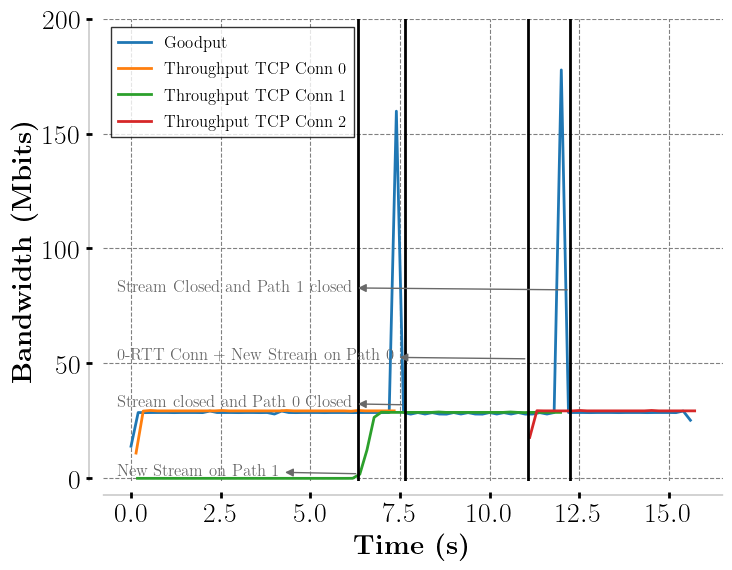
\includegraphics[scale=0.5]{figures/migration.png}
  \caption{Application-level connection migration during a 60MB file download}
  \label{fig:conn_migration}
\end{figure}


%-----------------------------------
\section{Research Agenda}\label{sec:research}
%-----------------------------------

% !TEX root = ./paper.tex
\label{sec:research}
By closely integrating \tcp and \tls, \tcpls opens new research questions
in the transport layer and above. We highlight some of these in this section.

\subsection{A More Secure Multipath TCP}

Multipath TCP \cite{rfc6824, rfc8684} is a recent TCP extension that allows a connection
to send data over different paths. It defines several \tcp options, including
\texttt{ADD\_ADDR} to advertise addresses and \texttt{RM\_ADDR} to remove addresses. Thanks to the \texttt{ADD\_ADDR} option, a dual-stack server can advertise
its IPv6 address over an IPv4 connection initiated by the client. The client can
then use this address to create an IPv6 subflow that is part of the same
connection.

One of the major deployments of Multipath TCP is on Apple's iPhones
\cite{bonaventure2016multipath}. This implementation has decided not to
support the \texttt{ADD\_ADDR} option for security reasons. Since the
Multipath TCP options are sent in clear, an attacker or
a malicious middlebox could try to hijack connections.
%The latest version
%of Multipath \tcp \cite{rfc8684} addresses this problem by including a
%HMAC in the new \texttt{ADD\_ADDR} option. However, this HMAC uses the key
%that is exchanged in clear during the connection handshake.
With \tcpls, this
security concern can be addressed elegantly. First, Multipath \tcpls
would not need to exchange a key in clear. It uses cookies (random 128-bits
bitstrings) sent as Encrypted Extensions in the ServerHello during the
handshake, and utilized in \tcpls \texttt{JOIN} handshakes.
Second, in the case of Multipath TCP, the \texttt{ADD\_ADDR} and
\texttt{RM\_ADDR} option could be sent inside \tls records that are encrypted and
authenticated. The information would then reach MP\tcp using a new
\texttt{setsockopt}. Furthermore, since the \tls records are part of the bytestream,
they are reliably delivered in contrast with the new \texttt{ADD\_ADDR} option
that is transmitted unreliably, like all \tcp options, and thus needs to be
echoed.

\subsection{A More Secure \tcp Fast Open}

\tcp Fast Open (TFO) \cite{rfc7413,radhakrishnan2011tcp} is another recent
\tcp extension that allows sending data inside the SYN. TFO defines a
\tcp option that encodes a cookie. This cookie is used to prevent attacks
from spoofed IP addresses. When a client connects first to a server, it sends
an empty cookie but no data in the SYN packet. The server computes a cookie
bound (e.g. using a hash) to the client's IP address and returns it
in the SYN+ACK. For subsequent connections, the client sends its cookie in the SYN
and places data in the payload. The server validates the cookie and processes
the data since it comes from a legitimate IP address. However, the \tcp header
length limits the size of the TFO cookie. \tcpls could easily include
a longer cookie inside the \tls ClientHello within the SYN
payload. This solution would reduce the number of options in the \tcp header
and provide stronger protections against attackers. With this change, \tcpls
would support a 0-RTT connection establishment similar to QUIC. In datacenters and controlled environments, this would work well. However, measurements
are required before deploying that approach in enterprise and
wireless networks as some of them contain middleboxes that block \tcp Fast Open
\cite{paasch2016network}. This middlebox interference has also affected QUIC \cite{langley2017quic} and is thus not specific to \tcp.


\subsection{Pluginizing \tcpls}

PQUIC~\cite{de2019pluginizing} proposed an elegant approach to deploy
QUIC extensions. Instead of waiting for new client and server implementations,
PQUIC includes an eBPF virtual machine to implement new features as bytecode
that can be exchanged over the QUIC connection.
%\tcpls could also be ``pluginized'' like Pluginized QUIC~\cite{de2019pluginizing}. In a nutshell, Plugizined QUIC is a QUIC implementation that includes an eBPF virtual machine and is structured to accept extensions in eBPF bytecode.
%This bytecode that implemnents new protocol features can be loaded from
%disk or exchanged using one the streams of an existing QUIC connection. This
%enables a QUIC server to dynamically push protocol extensions to its clients.

A \tcpls implementation could also be pluginized. The Linux kernel
already includes an eBPF virtual machine~\cite{ebpf:2014}.
It has already been used to develop several types of
\tcp extensions \cite{brakmo2017tcp, tran2019beyond, tran2020beyond}
and recent versions of the mainline kernel allow loading congestion control schemes implemented in eBPF bytecode. \tcpls can transport eBPF bytecode using
\tls records as a second non-data stream.
An interesting research question would be to evaluate the
limits of such a dynamic extensibility? A first intuition to make \tcp's
extensibility mechanism independent of the \tcpls version would be to let \tcpls
communicating plugins to handle new \tcp options and control behaviours, such that the
supported \tcp extensibility capability is not frozen by a given \tcpls
version, but rather dependent on the set of plugins exchanged.

\subsection{Limits to Cross-Layer Integration}

QUIC and \tcpls show that there are benefits in integrating protocols at
adjacent layers. QUIC already integrates HTTP/3~\cite{draft-ietf-quic-http},
but will likely be used by other
applications~\cite{draft-ietf-dprive-dnsoquic,ssh-quic}
in the future. \tcp and \tls are already used by a wide range of
applications~\cite{anderson2019tls}. Should \tcpls also be tuned
for specific applications such as HTTP/3? What are the critical differences
between QUIC and \tcpls from a functionality viewpoint?

%Finally, we would expect to critisize QUIC in light of our \texttt{\tcpls}
%design. We will compare both QUIC and \tcpls, discuss the differences, and analyze
%and answer questions regarding the requirements in transport protocol for today's
%Internet applications.



%\subsection{Plugizing \tcpls}


%Tran shown that the Linux \tcp implementation
%could also be extended using eBPF~\cite{tran2019beyond}. In addition to the
%socketA recent paper


%This could be added to our prototype, but a more interesting
%research question would be to define a generic API that any \tcpls
%implementation would implement and expose to eBPF

\subsection{Middlebox Interference}

As explained earlier, the deployment of recent \tcp extensions has been
hindered by various types of
middleboxes~\cite{detal2013revealing,medina2004measuring,hesmans2013tcp,edeline2017first}.
QUIC already suffered from such problems~\cite{langley2017quic}
and many implementations fall back to \tls over \tcp when blocked by a firewall.
Researchers and application developers could include middlebox detection
techniques inside \tcpls. Consider a \tcpls client that copies its \syn header
within a \tcpls message alongside the early data, or makes it part of the
zero-rtt resumption ticket message. By comparing the received \tcp header with
the original one, the server would immediately and reliably detect the presence
of NAT, transparent proxies or other types of middleboxes.  It could then inform
the client and adjust the configuration of their stacks accordingly or fall back
to regular \tcp to preserve connectivity. If deployed, such a protocol would
enable researchers to understand the impact of middleboxes more accurately.

\subsection{Efficient \tcpls Implementations}

During the last years, researchers have proposed
to move transport protocol implementations to user-space
\cite{jeong2014mtcp,marinos2014network} to
kernel bypass techniques such as netmap \cite{rizzo2012revisiting} or
DPDK. In parallel, parts of \tls moved to the Linux kernel
\cite{borkmanncombining} for performance reasons.
With new results on SmartNICs \cite{firestone2018azure}, it would be
interesting to analyze the best architecture for new \tcpls implementations.
Given the enormous efforts on implementing QUIC\cite{quicimplem},
it would be exciting
to compare QUIC and \tcpls from a performance viewpoint. From a protocol
standpoint, performance advantages of combining those two layers may be
achieved from, for example, adjusting the size of \tls records based on the
current \tcp congestion
window to avoid fragmented records (non-fragmented records makes \tcpls'
design having a zero-copy code path). More generally, we expect many performance
benefits from a more intertwined \tls/\tcp transport protocol at the
cost of design complexity.



%\subsection{What are the Limits of Cross-Layers Integration ?}

%QUIC is a recent example of an integrated protocol since it combines
%transport functions with \tls and application layer functions (HTTP/3). This
%integration can improve performance, but what are its drawbacks ?


%\newpage

%We expect to investigate several research questions with \tcpls. First, we are
%interested in analyzing how far we can go into supporting \tcp's extensibility
%through our mechanism. Several of new \tcp features may require to inject eBPF
%bytecode to the kernel. It is still unclear how much of \tcp could be extended,
%and if \texttt{\tcpls} may play a role in incentivizing the linux kernel's maintainer
%to support more eBPF in \tcp's implementation, since we now offer a technique to
%propagate eBPF bytecode within authenticated and confidential session with a
%trusted server.

%Second, we expect to analyze several features of \tcpls, such as our
%connection migration, our multipath implementation and our failover mechanism.
%Answering the question about how much \tcpls can or and how fast it performs in
%case of a migration or a network outage.



%\section{Implementation, Deployment \& Research Questions}

%% !TEX root = ./paper.tex

A \texttt{TCPLS} reference implementation is under active development. The
current implementation is forked from a fast and full
TLS 1.3 implementation written in \texttt{C}. It currently adds about 5k lines
of code (including unit tests and inline code comments) compared to the upstream branch.

The current implementation offers:
\begin{inparaenum}
  \item An experimental API that wraps TLS and TCP
  \item Our design of TCP's extensibility mechanism throught TCP option sent
within TLS records and processed by TCPLS. We currently support TCP User
Timeout and the injection of eBPF bytecode for TCP's congestion control
algorithm. Supporting another TCP option is only a matter of extending the sender's
API and processing the option
on the receiver side. TCPLS's internal machinery is already implemented for any
type of TCP option to send during the handshake or when the handshake completed.
  \item The support of parallel streams and multiplexing over TCP connections.
    Each stream has its own cryptographic context.
  \item Connection migration and multipathing.
\end{inparaenum}

We expect to investigate several research questions with TCPLS. First, we are
interested in analyzing how far we can go into supporting TCP's extensibility
through our mechanism. Several of new TCP features may require to inject eBPF
bytecode to the kernel. It is still unclear how much of TCP could be extended,
and if \texttt{TCPLS} may play a role in incentivizing the linux kernel's maintainer
to support more eBPF in TCP's implementation, since we now offer a technique to
propagate eBPF bytecode within authenticated and confidential session with a
trusted server.

Second, we expect to analyze several features of TCPLS, such as our
connection migration, our multipath implementation and our failover mechanism.
Answering the question about how much TCPLS can or and how fast it performs in
case of a migration or a network outage.

Finally, we would expect to critisize QUIC in light of our \texttt{TCPLS}
design. We will compare both QUIC and TCPLS, discuss the differences, and analyze
and answer questions regarding the requirements in transport protocol for today's
Internet applications.


%\section{Related Work}

%% !TEX root = ./paper.tex

By combining \tcp and \tls, \tcpls builds upon two of the most important
Internet protocols. Given their importance within  the research community and the IETF, we restrict our discussion to close related works. Readers may refer to survey papers for additional  context
information~\cite{polese2019survey,li2016multipath,papastergiou2016ossifying}.

Regarding its transport features, \tcpls' stream abstraction has similarities to
the Structured Streams Abstraction~\cite{ford2007structured}, in which each
stream does not need 3-way handshaking, is independent if attached to a
different \tcp connection and can proceed in parallel without head-of-line
blocking if the streams are not coupled. However, \tcpls pushes further the
abstraction, involving benefits leveraged from multiple connections.

\tcpls uses \tls records to encode data and control information. Researchers
have also explored the idea of encoding control information in the \tcp
bytestream in different protocols. During the initial discussions for Multipath \tcp, Multi-Connection \tcp (\texttt{MCTCP})~\cite{draft-scharf-mptcp-mctcp-01}
was proposed as an alternative that encodes control information in the bytestream. The \mptcp Working Group did not adopt this solution because it notably feared of possible problems with middleboxes. Multipath \tcp~\cite{raiciu2012hard,rfc8684} uses \tcp Options to encode control information and use different paths. \tcpls uses \tls records for this purpose and prevents middlebox tampering. Since \tls records are encrypted, their integrity protected, and protocol-level indistinguishable, middleboxes cannot interfere with the control information that \tcpls exchanges. In contrast, with \mptcp, a middlebox that modifies the payload, such as a transparent \tcp proxy or an application level gateway running on a NAT~\cite{rfc3027}, can disrupt the
protocol. Minion~\cite{nowlan2012fitting} also encodes control information in
the \tcp payload but to support unreliable data.

Given its security features, \tcpls must be compared with
\tcpcrypt~\cite{bittau2010case,rfc8548} which predates \tls 1.3. It uses \tcp
options to support opportunistic encryption but is not secure against an active
network attacker. \tcpls extends \tls while retaining its security  properties, 
and supporting new features. It is also compatible with middleboxes, as it 
leaves the \tcp wire format untouched.

%\tcpls also needs to be compared with
%\mptcp \cite{raiciu2012hard,rfc6824}.
\mptcp \cite{raiciu2012hard,rfc6824} supports several coupled congestion
control schemes \cite{peng2014multipath,wischik2011design,khalili2013mptcp}
that preserve fairness when different paths share the same bottleneck. A
similar solution  could be applied to \tcpls by leveraging eBPF to access and
modify the  congestion controller state. We leave this engineering effort as
future work. The initial idea of coupling \mptcp and \tls was proposed in an
Internet draft~\cite{draft-paasch-mptcp-ssl-00} that was not adopted by the
IETF. MPTCPSec~\cite{jadin2017securing} adds security capabilities to \mptcp but
comes with a large performance penalty.

Another important related work is \quic. %Its design has
%evolved over the years, and several companies adopted
%it~\cite{langley2017quic,Joras_mvfst,marx2020same}.
\quic version 1~\cite{rfc9000} also supports connection migration, but to our 
knowledge current implementations do not allow applications to trigger  it. 
%outside 
%from limited interoperability scripts.
%we could not test it in our lab since none of
%the available open-source implementations have implemented it yet.
Multipath extensions
\cite{viernickel2018multipath,de2017multipath,draft-liu-multipath-quic-02,I-D.lmbdhk-quic-multipath}
to \quic have been discussed but not yet adopted within the IETF. Finally,
\texttt{PQUIC}~\cite{de2019pluginizing} proposed to convey eBPF code over \quic
connections to deploy new protocol features. The same benefits are also being
considered for other distributed systems, such as BGP~\cite{xBGP} and
anonymous overlay networks~\cite{fan-hotpets}. This goes beyond the exchange of 
a congestion controller in \tcpls.

Finally, several solutions have been proposed to provide multipath capabilities
in the application layer. Examples include MP-H2~\cite{nikravesh2019mp} that
extends HTTP/2, MP-DASH~\cite{han2016mp} for video streaming or mHTTP~\cite{kim2014multi} that extends HTTP.

\tcpls also share similarities with \tls FOP~\cite{sy2020enhanced}, which
solves the privacy issue with TFO by using \tls. However, \tcpls is more 
generic, and its extensibility enables more advanced concerns and transport 
services.

%% Several researchers have proposed techniques to extend various transport
%% protocols. The IETF provides generic guidelines on the design of
%% protocol extensions \cite{rfc6709}. Several researchers have proposed
%% solutions to simplify the implementation of extensions to transport
%% protocols. The closest example include STP \cite{patel2003upgrading}, CTP
%% \cite{bridges2007configurable} and

%% Patel et al. \cite{patel2003upgrading} propose to use a type-safe version of C to extend a TCP
%% implementation by using bytecode. The implementation of TCPLS completely differs since it uses C to generate eBPF code. Furthemore, by leveraging the
%% flexibility of TLS, TCPLS can securrely exchange various options over a
%% connection. Bridges et al.
%% In CTP, Bridges et al. propose a new protocol that is composed of different microprotocols which can be combined together. In PQUIC, De Coninck et al. \cite{de2019pluginizing} include an eBPF virtual machine inside a QUIC implementation to extend it by using protocol plugins. Our approach is similar from an implementation viewpoint. By combining the TLS and TCP layers, we bring more extensibility to TCP.

%% %maybe
%% % ictcp \cite{wong2001configurable}

%% %configurable and extensible transport \cite{wong2001configurable}

%% % other protocols maybe

%% The IETF has developed various transport protocols, including
%% DCCP \cite{kohler2006designing}, SCTP \cite{rfc4960} and QUIC \cite{draft-ietf-quic-transport}. DCCP brings more flexible congestion control schemes

%% , lots of research but nothing related \cite{nowlan2012fitting}




%% % maybe
%% % Structured streams \cite{ford2007structured}


%% %TCP papers
%% %generic on extensibility

%% %tcp unreliable

%% A wide range of TCP extensions have been proposed \cite{rfc7414}. Some tune
%% protocol implementations with new strategies to retransmit lost data,
%% compute retransmission timers or manage congestion. These do not require
%% the definition of new TCP options that are negotiated during the handshake.
%% Some TCP extensions require the definition of new TCP options. These
%% include the timestamp and large windows extension \cite{rfc7313},
%% the support for selective acknowledgements \cite{rfc2018}, TCP Fast Open
%% \cite{rfc7413} or Multipath TCP \cite{rfc6824}. These extensions are negotiated
%% by exchanging TCP options during the connection handshake. These TCP options
%% allow to extend TCP, but they suffer from several limitations. First,
%% there is limited space in the TCP header to carry them. This limits the
%% number of extensions that can be used for a given TCP connection. The IETF
%% discusses solutions to extend the TCP header space, but the solution is neither
%% finalized nor implemented \cite{draft-ietf-tcpm-tcp-edo-10}. Second, middleboxes
%% interfere with the utilization of new options \cite{honda2011still}. This
%% interference severely limits the extensibility of TCP. TCPLS does not suffer
%% from these problems since the options that it carries are encrypted and can
%% span an entire TLS record (16KBytes).


%% % \cite{nowlan2012fitting}
%% %TODO
%% % idée de combiner des infos de TLS dans MPTCP
%% %\cite{draft-paasch-mptcp-ssl-00}
%% %\cite{jadin2017securing} % secure mptcp


%\section{Discussion}

%\input{discussion}


\section*{Software Artefacts}

A \texttt{TCPLS} reference documentation and implementation is under active development. The
current specifications and code are available on
\url{https://pluginized-protocols.org/tcpls}, forked from a fast and
full TLS 1.3 implementation written in \texttt{C}. Our \tcpls prototype adds
about 5k lines of C code to \texttt{picotls} latest version based on the latest
specification of TLS 1.3.

\section*{Acknowledgments}
We thanks the anonymous reviewers for their helpful feedback, and Mathieu Jadin
for its helpful guidance with IPMininet. This research is supported by the Walloon
Region through the ``Programme de recherche d'interet general
 WALINNOV" - MQUIC project (convention number 1810018).

